\section{Simulated Event Samples}%
\label{sec:tauid_mc}

The tau reconstruction and identification algorithms employed at the ATLAS
experiment for Run~2 of the LHC were developed using simulated events that
provide samples of \tauhadvis candidates. For \tauid, simulated
$\gammastar \to \tautau$ and dijet events are used, yielding samples of true
and \faketauhadvis, respectively.

% y->tautau:
% https://gitlab.cern.ch/atlas-physics/pmg/infrastructure/mc15joboptions/-/blob/master/share/DSID425xxx/MC15.425200.Pythia8EvtGen_A14NNPDF23LO_Gammatautau_MassWeight.py
An artificial $\gammastar \to \tautau$ event sample was generated
using \PYTHIA[8.212]~\cite{Sjostrand:2014zea} for the matrix element
calculation at leading order (LO), parton showering, hadronisation,
and \tauleptonC decays. The contribution of the $Z$ boson propagator to
the hard scattering process was removed to provide an unpolarised
sample of \tauleptons. In addition, the cross section of the process
was modified at generator-level to enhance the number of events with
high invariant $\tautau$ masses to increase the number of \tauhadvis
candidates with large transverse momenta. Both \tauleptons
are enforced to decay hadronically to minimise statistical
uncertainties from the size of the \truetauhadvisC sample.

% Di-jet samples: JZ1W up to JZ6W
% https://gitlab.cern.ch/atlas-physics/pmg/infrastructure/mc15joboptions/-/blob/master/share/DSID361xxx/MC15.361021.Pythia8EvtGen_A14NNPDF23LO_jetjet_JZ1W.py
Dijet events are generated using \PYTHIA[8.186]~\cite{Sjostrand:2014zea} for the
matrix element calculation at LO, parton showering, and hadronisation. The
generation is performed in slices of \pT of the leading jet (anti-\kt with
$R = 0.6$) constructed from generator-level particles. Slices with large jet
transverse momenta are oversampled to increase the number of events with jets
(\faketauhadvis) of large transverse momentum.

The $\gammastar \to \tautau$ and dijet samples use the A14 set of tuned
parameters for \PYTHIA[8]~\cite{ATL-PHYS-PUB-2014-021} and the
\NNPDF[2.3lo]~\cite{Ball:2012cx} set of parton distribution functions (PDFs).
Decays of hadrons containing $b$- or $c$-quarks are simulated using
\EVTGEN[v1.2.0]~\cite{Lange:2001uf}. The contamination of the hard scattering
interaction with soft, inelastic proton--proton collision events is accounted
for by overlaying the event with additional minimum-bias events. The response of
the ATLAS detector is simulated for all generated
events~\cite{SOFT-2010-01}. Subsequently, events are reconstructed from the
simulated detector response using the \textsc{Athena} software
suite~\cite{ATL-SOFT-PUB-2021-001}.


\subsection{\tauhadvis Candidate Selection}
\label{sec:tauid_candidate_selection}

The simulated events are used to construct samples of \tauhadvis candidates for
the development and performance evaluation of \tauid algorithms. Only candidates
passing the \tauhadvis reconstruction are considered and the following
selections are applied in addition:
\begin{itemize}

\item The number of \emph{core} tracks (\Ntracks) of the \tauhadvis candidate is
  either one or three. These are referred to as 1- or 3-prong \tauhadvis
  candidates, respectively.

\item The (visible) transverse momentum of the candidate needs to
  fulfil $\pT > \SI{20}{\GeV}$.

\item The \tauhadvis candidate needs to be within $|\eta| < 2.5$ but
  outside the transition region between barrel and end-cap
  electromagnetic calorimeters given by $1.37 < |\eta| < 1.52$.

\end{itemize}
In addition, reconstructed \tauhadvis candidates from
$\gammastar \to \tautau$ events are required to be geometrically
matched to a \tauhad at generator-level ($\Delta R < 0.2$).
% And the reco cuts are required to be fulfilled at truth-level.
All efficiencies and rejection factors given in the remainder of this
chapter do not include the effects of \tauhadvis reconstruction or the
selections outlined above.

The $\gammastar \to \tautau$ and dijet events provide samples of
true and \faketauhadvis with a size of 20 million and 46 million
candidates, respectively. The distributions of \tauhadvis candidate
\pT is shown for both samples and separately for 1- and 3-prong
candidates in~\Cref{fig:tauid_candidate_pt}. The difference in \pT
spectra between 1- and 3-prong \truetauhadvis in
\Cref{fig:tauid_candidate_pt_gammastar} results from a reduction in
track association efficiency for 3-prong \tauhadvis candidates with
increasing candidate \pT due to the decrease in angular separation of
charged hadrons from the \tauleptonC decay. In contrast, the \pT
spectrum of \tauhadvis candidates from dijet events, depicted in
\Cref{fig:tauid_candidate_pt_dijet}, shows a heavier tail towards
large \pT for 3-prong candidates due to the increase of the hadron
multiplicity in jets with jet \pT. For the development and performance
evaluation of \tauid algorithms, the sample of \faketauhadvis
candidates is re-weighted, separately for 1- and 3-prong candidates,
to match the \pT spectrum of \truetauhadvis from
$\gammastar \to \tautau$.

\begin{figure}[htbp]
  \begin{subfigure}{0.498\textwidth}
    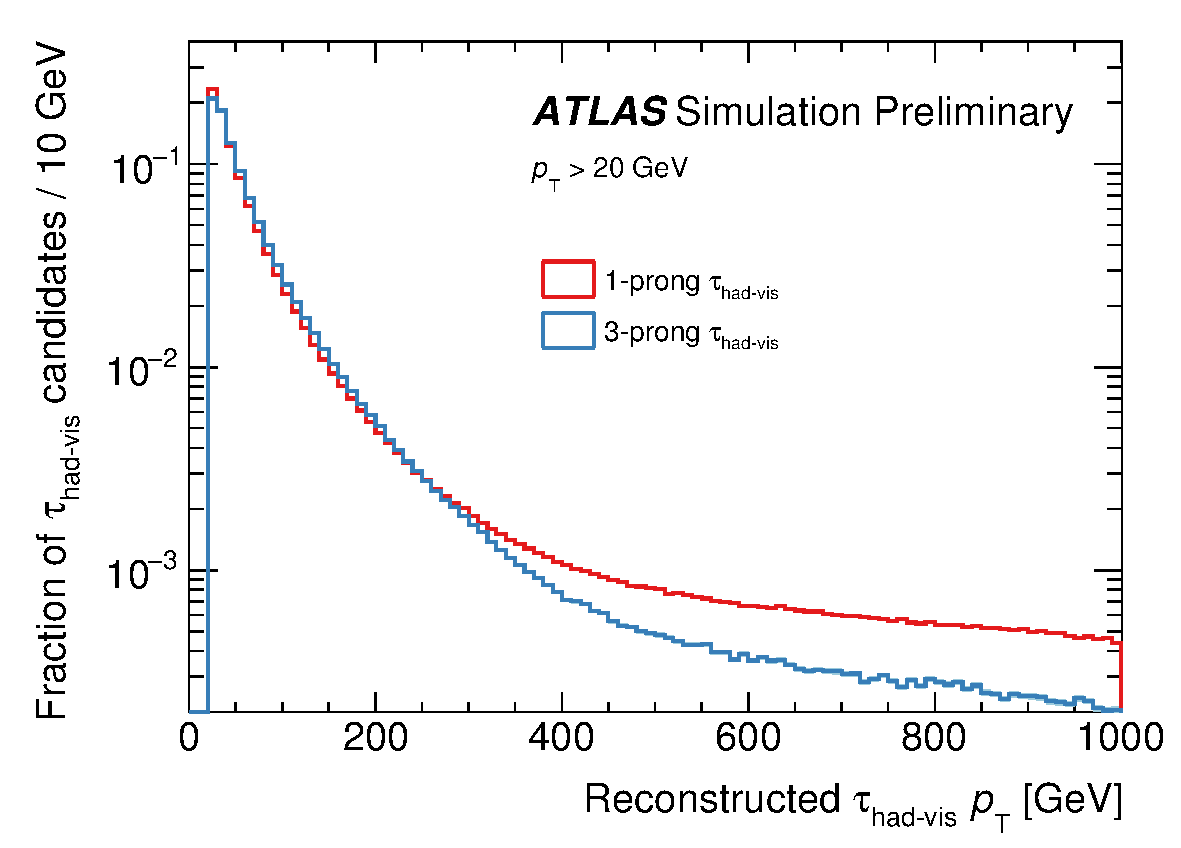
\includegraphics[width=\textwidth]{tauid/pubnote/taupt_gammastar}
    \subcaption{True-\tauhadvis from $\gammastar \to \tautau$ events}%
    \label{fig:tauid_candidate_pt_gammastar}
  \end{subfigure}\hfill%
  \begin{subfigure}{0.498\textwidth}
    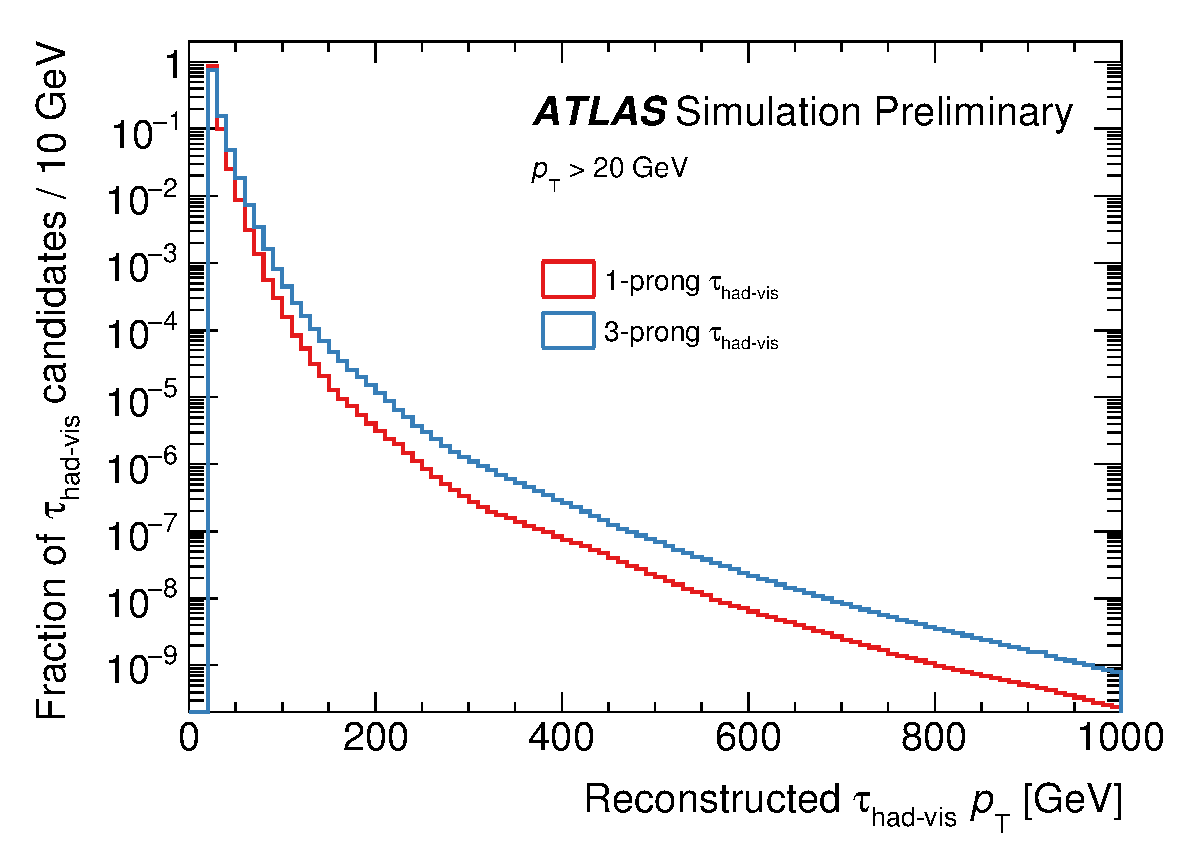
\includegraphics[width=\textwidth]{tauid/pubnote/taupt_dijet}
    \subcaption{Fake-\tauhadvis from dijet events}%
    \label{fig:tauid_candidate_pt_dijet}
  \end{subfigure}

  \caption[Transverse momentum distribution of \tauhadvis candidates in
  $\gammastar \to \tautau$ and dijet events.]{Transverse momentum distributions
    of 1- and 3-prong \tauhadvis candidates in $\gammastar \to \tautau$ (a) and
    dijet events (b). Statistical uncertainties are shown as coloured bands
    surrounding the central value. The figures are taken from
    Ref.~\cite{ATL-PHYS-PUB-2019-033}.}%
  \label{fig:tauid_candidate_pt}
\end{figure}


%%% Local Variables:
%%% mode: latex
%%% TeX-master: "../../phd_thesis"
%%% End:
